%**8-page Report Framework**
%
%1. Abstract (emphasize our variants)
%2. Introduction & Related Works (1 page)
%3. Formulation (1 page)
%4. Feature Extraction (2 pages)
%5. Learning (0.5 page)
%6. CRF Inference (0.5 page)
%7. Pixel Level result presentation (1 page)
%8. Result evaluation in rectangle level (1 page)
%9. Discussion (existing flaws and possible improvements) (0.5 page)
%10. acknowlegement and reference (0.5 page)
%
\documentclass[10pt,twocolumn,letterpaper]{article}

\usepackage{iccv}
\usepackage{times}
\usepackage{epsfig}
\usepackage{graphicx}
\usepackage{amsmath}
\usepackage{amssymb}

\DeclareMathOperator*{\argmin}{arg\,min}
\DeclareMathOperator*{\argmax}{arg\,max}
\newcommand{\SUM}{\sum\limits}
\newcommand{\hs}{\hspace{0.58in}}
% Include other packages here, before hyperref.

% If you comment hyperref and then uncomment it, you should delete
% egpaper.aux before re-running latex.  (Or just hit 'q' on the first latex
% run, let it finish, and you should be clear).
\usepackage[pagebackref=true,breaklinks=true,letterpaper=true,colorlinks,bookmarks=false]{hyperref}

\iccvfinalcopy % *** Uncomment this line for the final submission
\def\iccvPaperID{****} % *** Enter the ICCV Paper ID here
\def\httilde{\mbox{\tt\raisebox{-.5ex}{\symbol{126}}}}

% Pages are numbered in submission mode, and unnumbered in camera-ready
\ificcvfinal\pagestyle{empty}\fi
\begin{document}

%%%%%%%%% TITLE
\title{Application of Conditional Random Fields to Pixel-Level Salient Object Detection Through Local, Regional and Global Features}
%\title{Application of Conditional Random Field in Image Salient Object Detection\\ with Local, Regional and Global Feature Extraction}

\author{Jimmy Lin\\
Australian National University\\
Canberra, Australia\\
{\tt\small \url{linxin@gmail.com}}
% For a paper whose authors are all at the same institution,
% omit the following lines up until the closing ``}''.
% Additional authors and addresses can be added with ``\and'',
% just like the second author.
% To save space, use either the email address or home page, not both
\and
Christopher Claou\'e-Long\\
Australian National University\\
Canberra, Australia\\
{\small\url{u5183532@anu.edu.au}}
}

\maketitle
% \thispagestyle{empty}

%%%%%%%%% ABSTRACT
\begin{abstract}
    Making use of OpenCV, DARWIN and the MSRA dataset, we detect the saliency of by extracting local
    , regional and global saliency features at the pixel level, then combine those features with pre-fitted
    weights derived by logistic regression. The Conditional Random Field is then constructed to capture
    the spatial continuity of the saliency. The importance ratio of the combined unary and pairwise terms
    is determined by cross-validation. Based on the binary mask inferred by the Conditional Random Field,
    we ultimately apply a winner-takes-all algorithm to output a single bounding rectangle to label the
    detected salient object, by which the performance of our approach is evaluated through
    boundary-displacement error. 
\end{abstract}

%% Introduction & Related Works (1 page)
\section{Introduction and Motivation}
%{{{
A long-standing problem in the field of computer vision is how to calculate the saliency
of objects in an image -- that is, their prominence in the image when compared to their
background and surrounds.  This property is important for image recognition since it leads
to the ability to single out individual areas of an image, for example in automatic image
cropping and visual attention simulation in robotics, and 3D surface reconstruction in 
augmented reality displays.

\begin{center}
    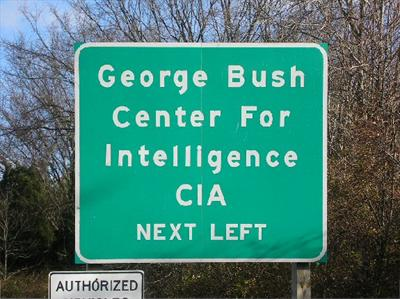
\includegraphics[width=0.6in,height=0.4in]{./Figures/example_image/4_140_140907.jpg}
    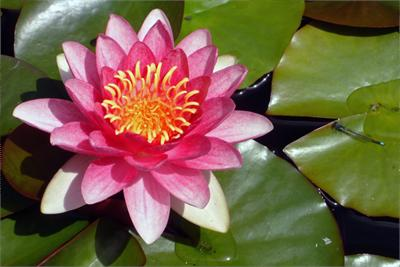
\includegraphics[width=0.6in,height=0.4in]{./Figures/example_image/4_141_141474.jpg}
    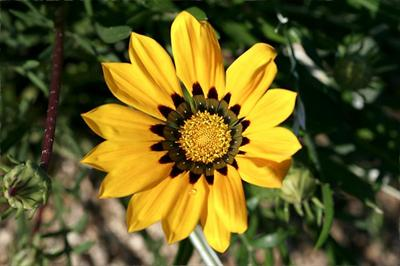
\includegraphics[width=0.6in,height=0.4in]{./Figures/example_image/4_141_141906.jpg}
    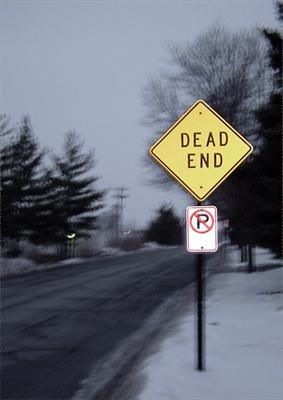
\includegraphics[width=0.6in,height=0.4in]{./Figures/example_image/4_142_142237.jpg}
    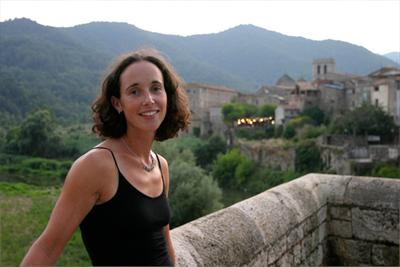
\includegraphics[width=0.6in,height=0.4in]{./Figures/example_image/4_142_142635.jpg}\\
    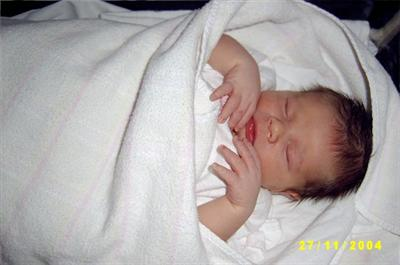
\includegraphics[width=0.6in,height=0.4in]{./Figures/example_image/4_124_124377.jpg}
    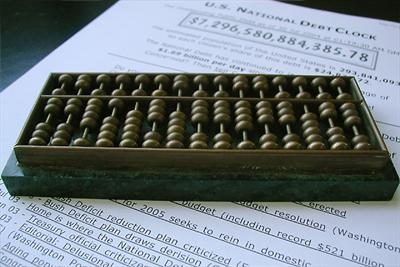
\includegraphics[width=0.6in,height=0.4in]{./Figures/example_image/4_124_124385.jpg}
    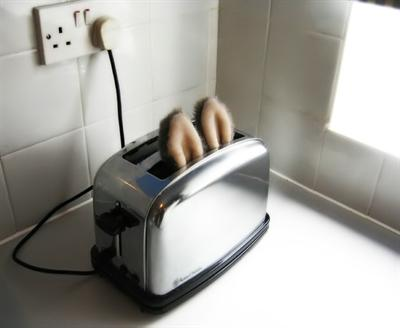
\includegraphics[width=0.6in,height=0.4in]{./Figures/example_image/4_124_124475.jpg}
    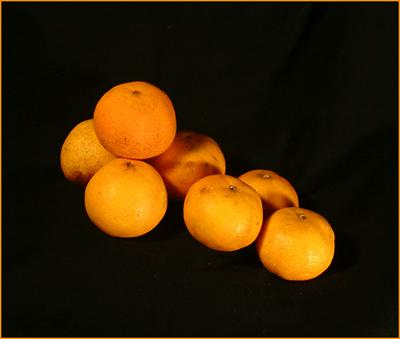
\includegraphics[width=0.6in,height=0.4in]{./Figures/example_image/4_124_124483.jpg}
    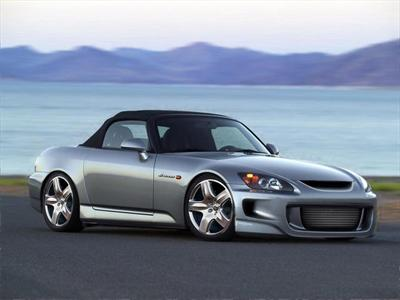
\includegraphics[width=0.6in,height=0.4in]{./Figures/example_image/4_128_128511.jpg} \\
    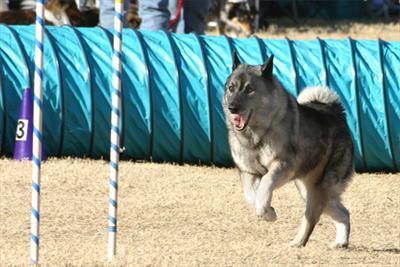
\includegraphics[width=0.6in,height=0.4in]{./Figures/example_image/4_129_129409.jpg}
    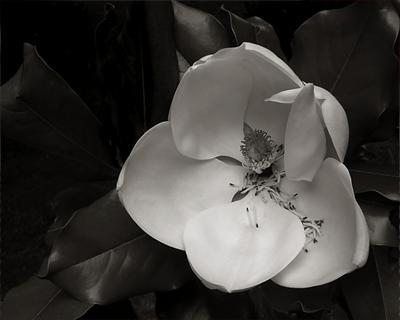
\includegraphics[width=0.6in,height=0.4in]{./Figures/example_image/4_132_132238.jpg}
    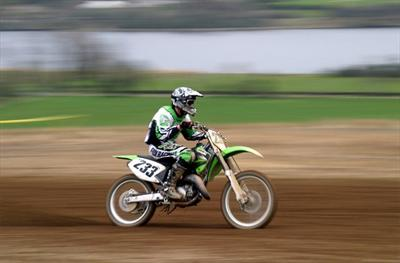
\includegraphics[width=0.6in,height=0.4in]{./Figures/example_image/4_135_135774.jpg}
    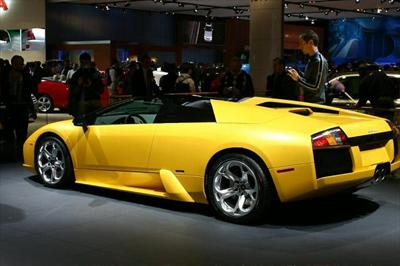
\includegraphics[width=0.6in,height=0.4in]{./Figures/example_image/4_136_136057.jpg}
    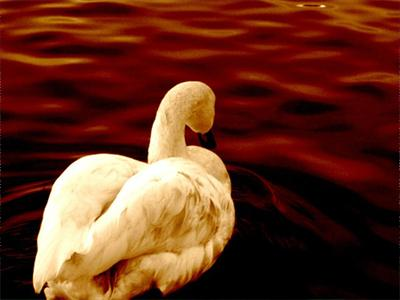
\includegraphics[width=0.6in,height=0.4in]{./Figures/example_image/4_136_136687.jpg}\\
    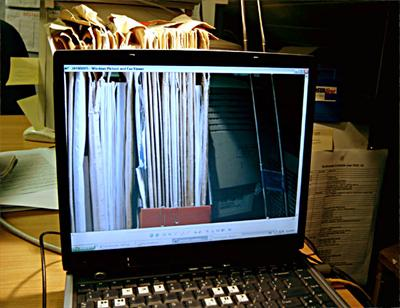
\includegraphics[width=0.6in,height=0.4in]{./Figures/example_image/4_137_137444.jpg}
    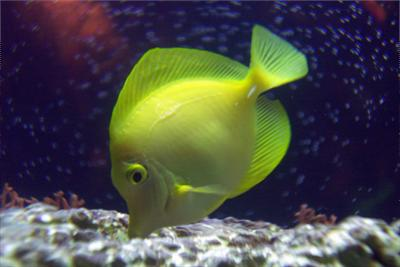
\includegraphics[width=0.6in,height=0.4in]{./Figures/example_image/4_138_138371.jpg}
    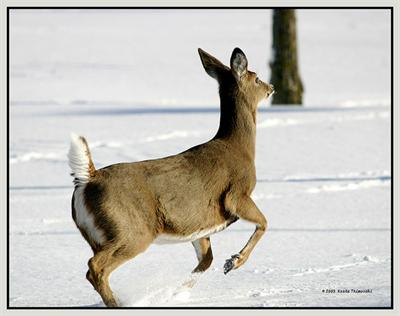
\includegraphics[width=0.6in,height=0.4in]{./Figures/example_image/4_139_139245.jpg}
    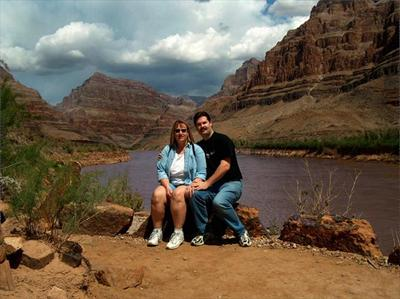
\includegraphics[width=0.6in,height=0.4in]{./Figures/example_image/4_139_139680.jpg}
    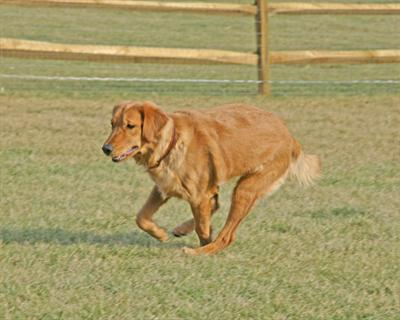
\includegraphics[width=0.6in,height=0.4in]{./Figures/example_image/4_140_140285.jpg}\\
    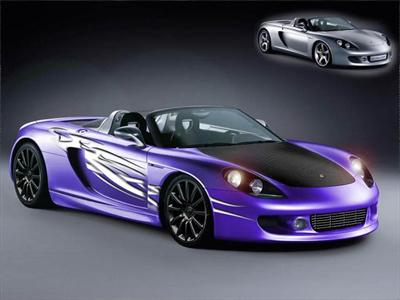
\includegraphics[width=0.6in,height=0.4in]{./Figures/example_image/4_142_142916.jpg}
    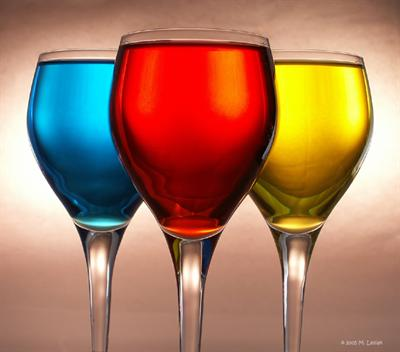
\includegraphics[width=0.6in,height=0.4in]{./Figures/example_image/4_143_143262.jpg}
    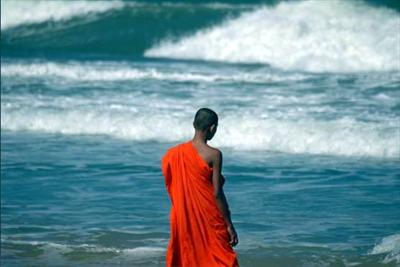
\includegraphics[width=0.6in,height=0.4in]{./Figures/example_image/4_144_144604.jpg}
    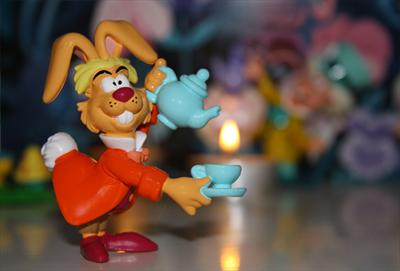
\includegraphics[width=0.6in,height=0.4in]{./Figures/example_image/4_134_134777.jpg}
    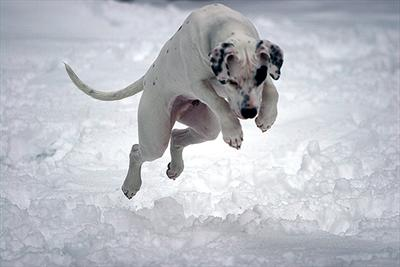
\includegraphics[width=0.6in,height=0.4in]{./Figures/example_image/4_134_134664.jpg}\\
    \footnotesize Fig. Example images from MSRA dataset B
    \end{center}
%}}}

%% Related Works (0.5 page)
\section{Related Works}
%{{{
Most existing visual attention approaches are based on the bottom-up computational framework,
where visual attention is supposed to be driven by low-level stimulus in the scene,
such as color intensity and contrast. These approaches consist of the following three steps:
The first step is feature extraction in which multiple low-level visual features, such as
intensity, color, orientation, texture, and motion, are extracted from the image at multiple
scales. The second step is saliency computation. The saliency is computed by a center-surround
operation, self-information, or graph-based random walk using multiple features. After
normalization and linear/nonlinear combination, a master map or a saliency map is computed
to represent the saliency of each image pixel. Last, a few key locations on the saliency map
are identified by winner-take-all, or inhibition-of- return, or other nonlinear operations.
%}}}

%% Formulation (1 page)
\section{Our Approach}

We base the essence of our salient object detection on several suppositions: 
it is likely for stuff with high contrast boundary to its near neighbours to be salient object, 
large "block" distinction relative to located surrounds, 
intensive colour distribution compared to all other color component
in candidate image and space continuity of saliency. \\

\subsection{Formulation}
%{{{
    To formulate the salient object detection problem, we incorporate the high-level concept
    of the salient object into the process of saliency map computation.
    As can be observed in Fig, people naturally pay more attention to salient objects in images, such as a person,
    a face, a car, an animal, or a road sign. Therefore, salient object detection can be formulated as a binary
    labeling problem that separates a salient object from the background. 

    For each pixel $x$ of given an image $I$, the binary mask $A_x$ indicate whether this pixel
    $x$ belongs to the salient object (1) or not (0). Thus, our objective can be transformaed to 
    derive the corresponding saliency map $A$, indicating binary salient property of one pixel.

    Build up a probabilistic model $P(A|I)=\frac{1}{Z}e^{-E(A|I)}$, where $\frac{1}{Z}$ is the normalising factor, and $E(A|I)$ is the energy function incorporating both unary and pairwise potentials between pixels.
    \begin{center}
        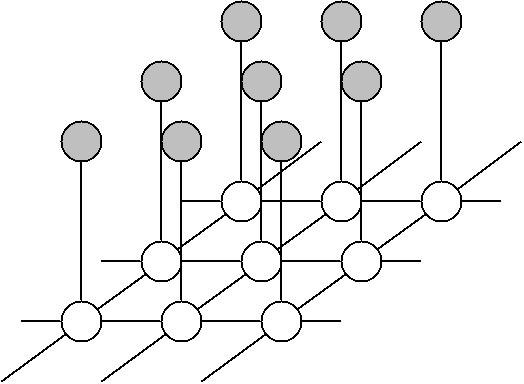
\includegraphics[width=1.8in,height=1in]{./Figures/mrf.jpg} \\
        \footnotesize Fig.2 graph for Conditional Random Field
        \end{center}



    Formally, the energy function can be represented as
    $$
    E(A|I) = \SUM_x S_{unary}(a_x,I) + \lambda_0 \SUM_{x,x'}S_{pair}(a_x,a_{x'},I)
    $$
    where $\lambda$ is the relative weight between the summary of multiple unary features and pairwise features. 

    The pairwise feature $S(a_x,a_{x'},I)$ exploits the spatial relationship between two adjacent pixels.  It can be viewed as a ``penalty'' for labelling adjacent pixels the same or differently.
    $$
    S(a_x,a_{x'},I) = |a_x-a_{x'}| \cdot e^{-\beta d_{x,x'}}
    $$
    where $x,x'$ represent two adjacent pixels, $d_{x,x'}$ is the L2-norm (standard norm) representing the colour difference between the two pixels, and $\beta=(2\langle||I_x-I_{x'}||^2\rangle)^{-1}$ is a robust parameter to weight the colour contrast.
    
    The unary potential for combination of three features is specified as 
    $$
    S_{unary}(a_x,I) = \SUM_{k=1}^K \lambda_k \cdot F_k(a_x,I)
    $$
    where $\lambda_k$ is the weight of the $k^{th}$ feature conforming to $\sum_{k=1}^{K} \lambda_k = 1$.
    \begin{center} %% image 5_156_156422
    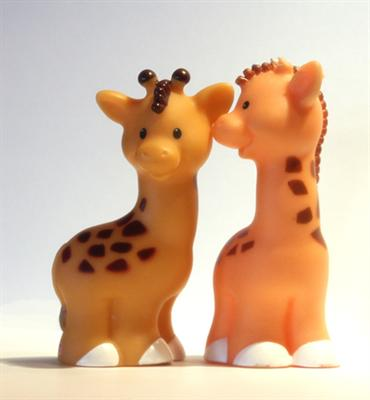
\includegraphics[width=0.6in,height=0.8in]{./Figures/previews/raw.jpg}
    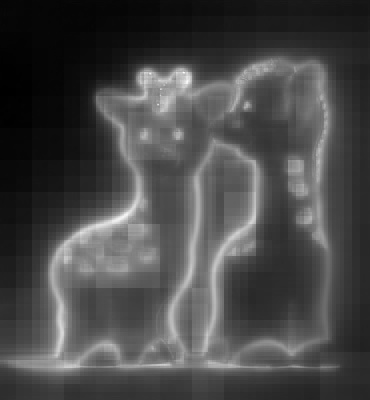
\includegraphics[width=0.6in,height=0.8in]{./Figures/previews/MC.jpg}
    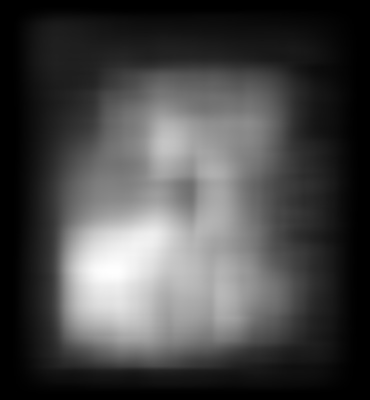
\includegraphics[width=0.6in,height=0.8in]{./Figures/previews/CSH.jpg} 
    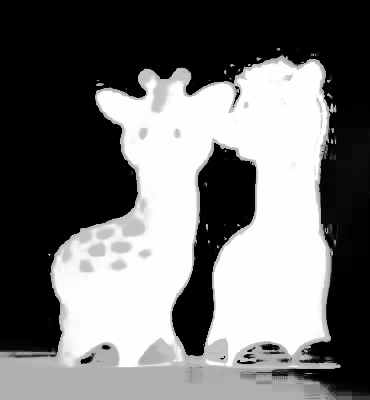
\includegraphics[width=0.6in,height=0.8in]{./Figures/previews/CSD.jpg} 
    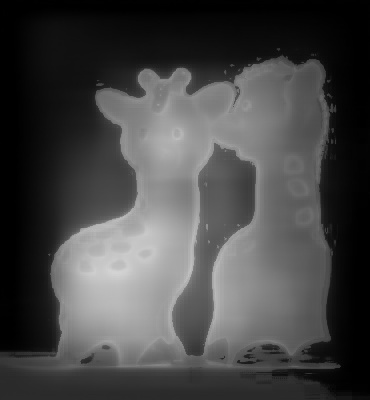
\includegraphics[width=0.6in,height=0.8in]{./Figures/previews/Composed.jpg} \\
    {\footnotesize Fig.3 Original Image and Preview of feature maps \\ 
       Left to Right: (b) multiscale contrast  (c) center surround histogram \\[-1mm] 
    (d) color spatial distribution (e) composed unary potential}
    \end{center}
    The value of each feature $F_k(a_x,I)$ comes from a normalised feature map $f_k(x,I)\in[0,1]$, and for each pixel:
    $$
    F_k(a_x,I) = \left\{\begin{matrix}f_k(x,I), & a_x=0\\1-f_k(x,I), & a_x=1\end{matrix}\right. 
    $$
%}}}

%% Feature Extraction (2 pages)
\subsection{Feature Extraction}
Feature Extraction, widely acknowledged as the most significant component of computer vision task,
represents how we want the computer to interpret the raw iamges. In this project, we just focus
on three critical features, each of which is capable of capturing the saliency individually but
in various level of scope. They are respectively Multiscale Contrast, Center Surround Histogram 
and Color Spatial Distribution. 
%% local feature
\subsubsection{Multiscale Contrast}
%{{{
Constrast is commonly utilised as local feature because the contrast operator simulates
the human visual receptive fields. Specifically, it captures the point that salient object
tends to have tremendous contrast to the surroundings in its boundary (not vice versa).
Since we may have no preknowledge about the size of salient object, it is usual
to compute the contrast at multiple scale. 
% TODO ADD detailed analysis about why we should have multiple scales.

    \begin{center}    
        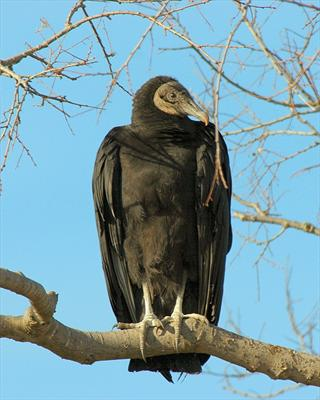
\includegraphics[width=0.65in,height=0.9in]{./Figures/pyramid/5_145_145839raw.jpg} \hspace{2mm}
    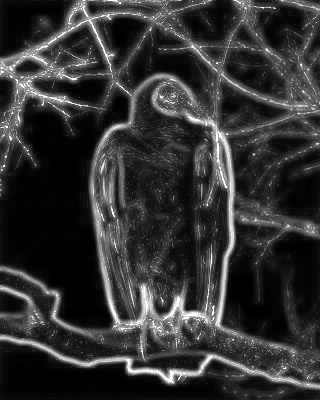
\includegraphics[width=0.65in,height=0.9in]{./Figures/pyramid/5_145_145839_p0.jpg} 
    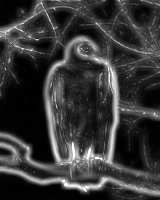
\includegraphics[width=0.325in,height=0.45in]{./Figures/pyramid/5_145_145839_p1.jpg} 
    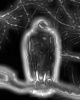
\includegraphics[width=0.1625in,height=0.225in]{./Figures/pyramid/5_145_145839_p2.jpg} 
    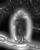
\includegraphics[width=0.08125in,height=0.1125in]{./Figures/pyramid/5_145_145839_p3.jpg} 
    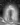
\includegraphics[width=0.040625in,height=0.0575in]{./Figures/pyramid/5_145_145839_p4.jpg} 
    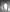
\includegraphics[width=0.0203125in,height=0.02825in]{./Figures/pyramid/5_145_145839_p5.jpg} \hspace{1mm}
    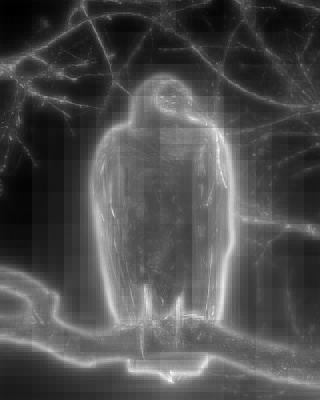
\includegraphics[width=0.65in,height=0.9in]{./Figures/pyramid/5_145_145839.jpg} \\
    \footnotesize Fig. Pyramid of Multiscale Contrast.  \\
    (a) leftmost: Original Image. (b) rightmost: Multiscale Feature Map. \\
    (c) immediate images: multiscale pyramids from level $1$ to $6$.
    \end{center}

Hence, define the multiscale constrast to be 
a contrast map from the linear combination of image contrast at all levels of an N-level
gaussian image pyramid, using the pixels $x$ in the image $I$:
    $$
    f_c(x,I) = \SUM_{n = 1}^{N}\SUM_{x'\in W(x)}||I^n(x)-I^n(x')||^2
    $$
where W(x) is a window that delineates which area to consider for neighbouring pixels to compare contrast values.

% TODO ADD explanation for why we need to choose such window size and pyramid level.
In our implementation, we choose the total number of pyramid level $N$ to be $6$ and 
the size of the window to be $9 \times 9$. 

It is evident that the Multiscale Contrast give high distinction between the boundary and non-boundary region. 
This provides us a precise description of where the boundary of salient object exist in the output binary mask.
For those salient object has relatively large contrast within its body, this feature works perfectly, such as 
the bird in the second image and the house in the third image. 
As to the pixels within the salient objects, they are usually given low marks, this weakness can be complemented
by the regional feature - Center Surround Histogram, which will be introduced latter.

    \begin{center}
    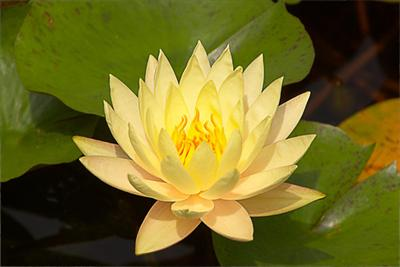
\includegraphics[width=0.7in,height=0.54in]{./Figures/contrast/1orig.jpg}
    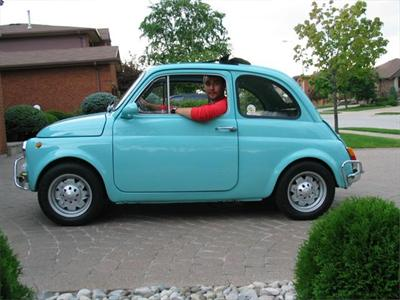
\includegraphics[width=0.7in,height=0.54in]{./Figures/contrast/2orig.jpg}
    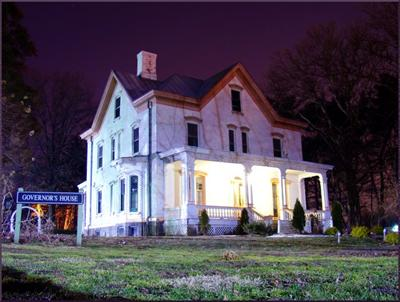
\includegraphics[width=0.7in,height=0.54in]{./Figures/contrast/3orig.jpg}
    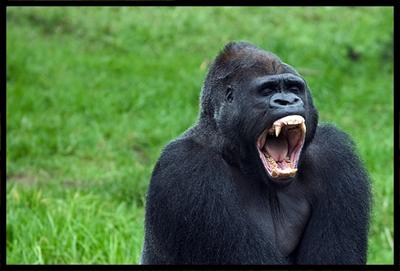
\includegraphics[width=0.7in,height=0.54in]{./Figures/contrast/4orig.jpg}\\
    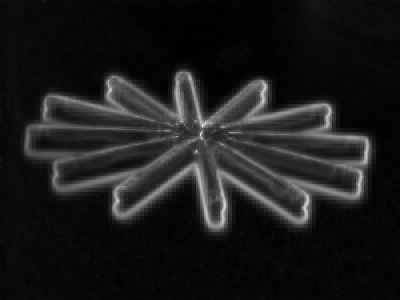
\includegraphics[width=0.7in,height=0.54in]{./Figures/contrast/1cont.jpg}
    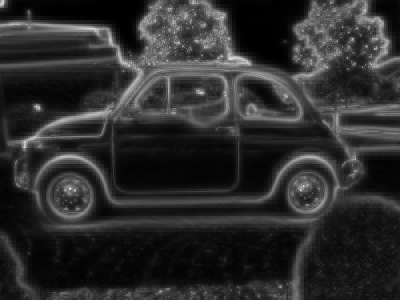
\includegraphics[width=0.7in,height=0.54in]{./Figures/contrast/2cont.jpg}
    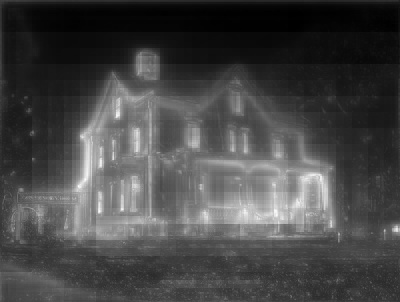
\includegraphics[width=0.7in,height=0.54in]{./Figures/contrast/3cont.jpg}
    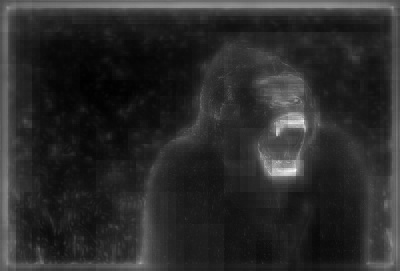
\includegraphics[width=0.7in,height=0.54in]{./Figures/contrast/4cont.jpg}\\
    \footnotesize \hspace{0.1cm} (a) \hs (b) \hs  (c) \hs (d) \\
     Fig. Feature Maps of Multiscale Contrast under various scenes
    \end{center}

But there are some drawbacks that are tough to avoid. 
First and foremost, boundary of all objects are highlighted, which is obviously not desired.
We only wish to give high mark to pixels that are relavant to salient object, rather than all boundaries in one image. 
This would possibly lead to some "saliency leak" in the ultimate result and deteriorate detection precision
 since some pixels outside the true salient object are likely to be considered as a part of that object.

Bad vulnerability to the outlier pixels within the body of salient object is another problem of multiscale contrast. 
Look at the chimpanzee in the fourth image, the tooth is tremendously contrasted to its surroundings,
far beyond the contrast of the body of chimpanzee to the grass. Since each entry of output feature map 
is quantitatively normalised, the contrast of the body of chimpanzee to the grass is comparatively trivial.
However, the tooth may be too narrow to be observed by the human receptive field and thus not 
labelled as the salient object. That is, this flaw may result in the low recall comparing to the ground truth data.%}}}

\subsubsection{Center Surround Histogram}
%% regional feature
%{{{
    As shown in the Fig. , the local feature - multiscale contrast only partially detects salient objects 
since it is only sensitive to the boundaries. Out of the purpose of detecting the whole block of objects,
we make use of another static salient feature, which captures the regional information of saliency  
and can be computed using various low-level features via a center-surround operation. 

Create a colour RGB histogram for both the rectangle and the surrounding frame, 
which has the same area with the center rectangle, with a certain resolution 
(number of ``bins'' for each colour). And then measure the distinguishability of the 
area centered at each pixel $x$ 
by calculating the $\chi^2$ value between the two histograms to obtain the differences 
between the rectangle and the surrounding frame.  Do this for multiple aspect ratios, 
and keep the largest $\chi^2$ value: 

    \begin{align*}
    R(x) &= \argmax\limits_{R(x)}\chi^2(R(x), R_s(x)) \\ &=\argmax\limits_{R(x)}\frac{1}{2}\cdot\SUM_{i\in bins}\frac{(hist_{R(x)_i}-hist_{R_s(x)_i})^2}{hist_{R(x)_i}+hist_{R_s(x)_i}}
    \end{align*}
    
    Here, we traverse through five template of rectangle with different aspect ratio 
    $\{ 0.5, 0.75, 1.0, 1.25, 1.5\}$ for determining the most distinct pair of center 
    and surround rectangle centered at each pixel $x$. Besides, to reduce the demands 
    on computational resources, the size range of the rectangle is discretized to be 
    12 ratios $\{ {0.18, 0.2, 0.25, 0.3, 0.35, 0.4, 0.45, 0.5, 0.55, 0.6, 0.65, 0.7, 0.75}\}$
    with regards to  $min(w,h)$, which is the minimal value of width and height of 
    the processed image.

    The center-surround histogram feature at each pixel $x$ is finally calculated by:
    $$
    f_h(x,I)\propto\SUM_{x'|x\in R(x')}w_{xx'}\chi^2(R(x'),R_s(x'))
    $$
    Note that the center-surround histogram feature reflects the distinguishability of 
    each pixel, which is assigned from the distinguishability of the most outstanding 
    area centered at each pixel of one image, with the weight of spatial closeness
    to the center of that area. 

    \begin{center}
    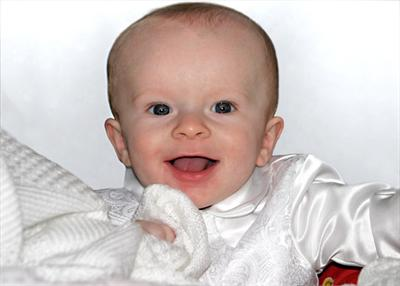
\includegraphics[width=0.7in,height=0.54in]{./Figures/CSH_image/1orig.jpg}
    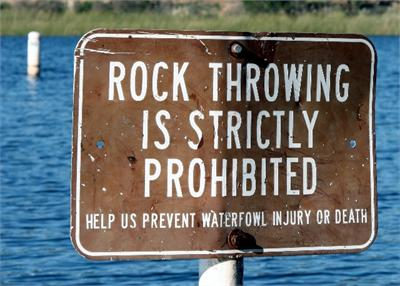
\includegraphics[width=0.7in,height=0.54in]{./Figures/CSH_image/2orig.jpg}
    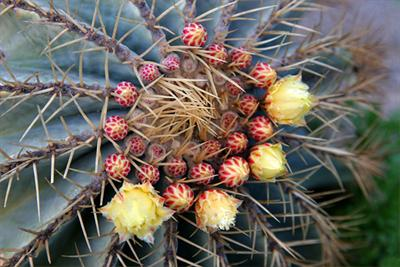
\includegraphics[width=0.7in,height=0.54in]{./Figures/CSH_image/3orig.jpg}
    \includegraphics[width=0.7in,height=0.54in]{./Figures/CSH_image/4orig.jpg}\\
    \includegraphics[width=0.7in,height=0.54in]{./Figures/CSH_image/1cont.jpg}
    \includegraphics[width=0.7in,height=0.54in]{./Figures/CSH_image/2cont.jpg}
    \includegraphics[width=0.7in,height=0.54in]{./Figures/CSH_image/3cont.jpg}
    \includegraphics[width=0.7in,height=0.54in]{./Figures/CSH_image/4cont.jpg}\\
    \footnotesize \hspace{0.1cm} (a) \hs (b) \hs  (c) \hs (d) \\
    Fig. Feature Maps of Center-Surrond Histograms under various scenes
    \end{center}

    %% TODO advantage and drabacks of this feature.
    As we can see from above Fig, the whole salient block within one image is given distinguishable 
    emphasis comparing to its surrounds in the output feature map. 


%}}}

%% global feature
\subsubsection{Color Spatial Distribution}
%{{{
    The goal of using Color Spatial Distribution feature is to take into account the global saliency information, 
    that is, the information about how widely the colors occurring in one image are distributed over the global scope.
    By creating Gaussian Mixture Components and fitting them to pixels of the whole image, the
    variance of each color component can be captured and we give penality to the pixels with high-variance 
    color according to the supposition that the colour of salient object in one image tends to have 
    intensive spatial distribution.
    
    According to the theory of Machine Learning, each pixel is associated to a colour component with the probability
    $$
    P(c|I_x) = \frac{\omega_c\mathcal{N}(I_x|\mu_c,\Sigma_c)}{\SUM_c \omega_c \mathcal{N}(I_x|\mu_c,\Sigma_c)}
    $$
    where $\omega_c$ is the weight, $\mu_c$ is the mean colour, $\Sigma_c$ is the covariance, and $\mathcal N(I_x|\mu_c,\Sigma_c)$ is the multivariate normal distribution of the $c^{th}$ component.

    For each fitted gaussian color component $c$, we compute its horizontal variance $V_{h}(c)$ as follows,
    $$
    V_{h}(c) = \frac{1}{|X|_{c}} \sum_{x} p (c|I_{x}) \cdot | x_{h} - M_{h}(c) |^{2}
    $$
    where $x_h$ is horizontal coordinate of pixel $x$, $|X|_c$ is normalising factor 
    and $M_h (c)$ is the mean of the gaussin component:
    $$
    |X|_c = \sum_x p(c|I_x)
    $$
    $$
    M_h (c) = \frac{1}{|X|_c} \sum_{x} p(c|I_x) \cdot x_h
    $$

    Vertical variance $V_{v}(c)$ is defined similiarly, and we equally combine the horizental and vertical variance to derive the unnormalised composite variance $V_h (c)$: 
    $$
    V' (c) = V_h (c) + V_v (c) 
    $$

    Then employ the min-max approach to normalise the composite covariance:
    $$
    V (c) = \frac{V'(c) - min \big(V'(c)\big) }{max \big(V'(c)\big) - min \big(V'(c)\big)}  
    $$
    where $V(c)$ is the normalised composite covariance of the $c^{th}$ component, contained between 0 and 1.

    The final colour spatial distribution feature for pixel $x$ is defined as a weighted sum of its color intensiveness:
    $$
    f_s(x,I)\propto\SUM_c p(c|I_x)\cdot(1-V(c))
    $$

    The feature map $f_s (\cdot,I)$ is also normalized to the range $[0, 1]$. The following figure
    shows color spatial-distribution feature maps of several example images. 
    The salient objects are well covered by this global feature. 

    \begin{center}
    \includegraphics[width=0.72in,height=0.52in]{./CSD_image/1.jpg}
    \includegraphics[width=0.72in,height=0.52in]{./CSD_image/2.jpg}
    \includegraphics[width=0.72in,height=0.52in]{./CSD_image/3.jpg}
    \includegraphics[width=0.72in,height=0.52in]{./CSD_image/4.jpg}\\
    \includegraphics[width=0.72in,height=0.52in]{./CSD_image/1_CSD.jpg}
    \includegraphics[width=0.72in,height=0.52in]{./CSD_image/2_CSD.jpg}
    \includegraphics[width=0.72in,height=0.52in]{./CSD_image/3_CSD.jpg} 
    \includegraphics[width=0.72in,height=0.52in]{./CSD_image/4_CSD.jpg} \\
    \footnotesize \hspace{0.1cm} (a) \hs (b) \hs  (c) \hs (d) \\
     Fig. Feature Maps of Color Spatial Distribution under various scenes
    \end{center}

    % why it is a successful feature in detecting the saliency
    It is evident that the global feature gains a huge success in mark up the saliency when the background
    is monotonous. As illustrated by the first three images in the above figure, the flying stuff
    is distinguished from the bichrome background - blue ocean and white tide, the sign card under the 
    background of ocean and tree leaves and in the third image the girl body before the fully white wall.
    % Weaknesses of this feature
    However, in the case of colorful background, color spatial distribution, with a high probability,
    fails to distinguish the salient object in the image. The Fig.. (d) demonstrates us
    this undesired property of the global feature. 

    % our variation
    One variation in our implementation is to create the component model from only a subset of the pixels in the image.
    The pixels in the subset is picked up with equal spatial distance. Specifically, we apply the "pydown" module 
    in Opencv to dilute the pixels participating this unsupervised learning task.
    Such manipulation will not sacrifice too much accuracy, but greatly reduce 
    the running time of fitting the Mixture of Gaussians since the number of pixels provided for the fitting halves. 

    \begin{center}
    \includegraphics[width=0.72in,height=0.52in]{./Figures/pydownCompare/1.jpg}
    \includegraphics[width=0.72in,height=0.52in]{./Figures/pydownCompare/1NOPYDOWN.jpg}
    \includegraphics[width=0.72in,height=0.52in]{./Figures/pydownCompare/1PYDOWN.jpg} 
    \includegraphics[width=0.72in,height=0.52in]{./Figures/pydownCompare/1DOUBLEPYDOWN.jpg} \\
    \includegraphics[width=0.72in,height=0.52in]{./Figures/pydownCompare/2.jpg}
    \includegraphics[width=0.72in,height=0.52in]{./Figures/pydownCompare/2NOPYDOWN.jpg}
    \includegraphics[width=0.72in,height=0.52in]{./Figures/pydownCompare/2PYDOWN.jpg} 
    \includegraphics[width=0.72in,height=0.52in]{./Figures/pydownCompare/2DOUBLEPYDOWN.jpg} \\
    \includegraphics[width=0.72in,height=0.52in]{./Figures/pydownCompare/3.jpg}
    \includegraphics[width=0.72in,height=0.52in]{./Figures/pydownCompare/3NOPYDOWN.jpg}
    \includegraphics[width=0.72in,height=0.52in]{./Figures/pydownCompare/3PYDOWN.jpg} 
    \includegraphics[width=0.72in,height=0.52in]{./Figures/pydownCompare/3DOUBLEPYDOWN.jpg} \\
    \footnotesize (a) original (b) no pydown (c) one-level pydown (d) two-level pydown
    Fig. Examples for global feature using diluted images \\
    \end{center}

    We test three levels of pixel dilution: no pydown, one-level pydown and two-level pydown. One-level
    pydown means reducing both of the width and height of one image to half of the original size, 
    such that only a quarter of pixels are available for fitting the mixture of gaussians.
    From the above figure, it is evident that one-level pydown, to some extent, increases the quality of 
    this global feature by marking the salient block softly or obscurely rather than in a strict way. 
    Extraction for two-level pydown 
    indicated in Fig. (d) is even faster, but generally it lost the effectiveness of this global feature.
    Hence, in our implementation of color spatial distribution, we employ the one-level pydown as a trick
    to both enhance quality of global feature and improve extraction time performance.

    Besides, the maximum number of iterations is limited $(100)$ and the convergence criterion is lowered $(10^{-1})$
    in order to reduce the time taken to compute this feature.  This outcome of this global feature, after such
    simplification, will not get deteriorated since we only care about capturing 
    approximate component location, rather than precisely maximum likelihood of the coloured pixels.

    The number of gaussian components is another trade-off between the quality of feature extraction
    and computational cost. Our implementation uses five gaussians to softly capture color components in one image. 
%}}}

%% Learning (0.5 page)
\subsection{Learning}
Those three features aforementioned have their own strengthes and weaknesses in different areas. For example, the .
It goes without saying that incorporating all three features into the unary potential of the CRF model 
to complement each other. It would be oversimplistic and unpersuasive to treat three features in equal weight 
since one feature perhaps may be stronger than other two features and ought to be assigned with higher importance.
Hence, one effective and reasonable approach is to adjustably determine the optimal weight to combine three features
with the help of certain machine learning algorithm. 

In this project, we implement logistic regression to decide the optimal weight under the help of training data.

%% CRF Inference (0.5 - 1 page)
%% images for inferred binary mask
\subsection{CRF Inference}
To infer the maximum likelihood assignment for pixelwise variables under the CRF framework,
the usual message passing algorithm would be intractable. Therefore, we turn to the $\alpha$-expansion inference,
which successively segments all and non-$\alpha$ pixels with graph cuts and the algorithm will 
change the value of $\alpha$ at each iteration with graph-cut algorithm. 
By this means, inferring maximum likelihood assignment for binary saliency variable, or equivalently, 
 minimal energy function would be much faster. 

But how to determine the parameter $\lambda_0$, which indicates to what extent, relative to the 
unary term (combined feature map), we ought to consider the pairwise potential in 
deciding the binary saliency of one pixel? And this parameter would influence the smoothness of
resulting binary mask since pairwise term can be regarded as the penality to adjacent pixels 
with different labels. Our solution is to determine the optimal $\lambda_0$
by applying the cross validation on $\lambda_0$ at various magnitudes. 

%% TODO add diagram and graph to illustrate our cross validation on various lambda
TODO:add diagram and graph to illustrate our cross validation on various lambda \\

By cross validation above, the optimal parameter $\lambda_0$ we use for evaluating the binary mask is 8.
\begin{center}
    \includegraphics[width=0.8in,height=0.6in]{./Figures/CRFinference/5_159_159364.jpg}
    \includegraphics[width=0.8in,height=0.6in]{./Figures/CRFinference/5_159_159364_3.jpg}
    \includegraphics[width=0.8in,height=0.6in]{./Figures/CRFinference/5_159_159364_2.jpg} \\
    \includegraphics[width=0.8in,height=0.6in]{./Figures/CRFinference/5_159_159649.jpg}
    \includegraphics[width=0.8in,height=0.6in]{./Figures/CRFinference/5_159_159649_3.jpg}
    \includegraphics[width=0.8in,height=0.6in]{./Figures/CRFinference/5_159_159649_2.jpg} \\
    \includegraphics[width=0.8in,height=0.6in]{./Figures/CRFinference/5_162_162349.jpg}
    \includegraphics[width=0.8in,height=0.6in]{./Figures/CRFinference/5_162_162349_3.jpg}
    \includegraphics[width=0.8in,height=0.6in]{./Figures/CRFinference/5_162_162349_2.jpg} \\
    \footnotesize  (a) Raw Image (b) Combined Unary Map  (c) Binary Mask ($\lambda=8$)\\
     Fig. Examples for CRF inference by $\alpha$-algorithm
\end{center}

%% Result evaluation in rectangle level (1 page)
%% images for the output rectangle
\section{Result Evaluation}
We randomly pick up 500 images from MSRA dataset B to form the training set. And we choose another 500 images
to form the testing set.
\subsection{Bounding Box}
The binary mask, derived from the CRF inference, can be directly used for various applications. 
However, in order to evaluate the effectiveness of our approach, we make use of ... algorithm to output a bounding 
rectangle to box the salient object, based on the derived pixelwise binary mask. 

%% TODO Specific algorithm for output bounding box

\begin{center}
    \includegraphics[width=0.6in,height=0.4in]{./Figures/boundingbox/5_145_145114RECT.jpg}
    \includegraphics[width=0.6in,height=0.4in]{./Figures/boundingbox/5_145_145275RECT.jpg}
    \includegraphics[width=0.6in,height=0.4in]{./Figures/boundingbox/5_145_145349RECT.jpg}
    \includegraphics[width=0.6in,height=0.4in]{./Figures/boundingbox/5_145_145398RECT.jpg}
    \includegraphics[width=0.6in,height=0.4in]{./Figures/boundingbox/5_146_146319RECT.jpg} \\
    \includegraphics[width=0.6in,height=0.4in]{./Figures/boundingbox/5_146_146330RECT.jpg}
    \includegraphics[width=0.6in,height=0.4in]{./Figures/boundingbox/5_146_146332RECT.jpg}
    \includegraphics[width=0.6in,height=0.4in]{./Figures/boundingbox/5_146_146431RECT.jpg}
    \includegraphics[width=0.6in,height=0.4in]{./Figures/boundingbox/5_146_146552RECT.jpg}
    \includegraphics[width=0.6in,height=0.4in]{./Figures/boundingbox/5_147_147367RECT.jpg} \\
    \includegraphics[width=0.6in,height=0.4in]{./Figures/boundingbox/5_148_148067RECT.jpg}
    \includegraphics[width=0.6in,height=0.4in]{./Figures/boundingbox/5_148_148271RECT.jpg}
    \includegraphics[width=0.6in,height=0.4in]{./Figures/boundingbox/5_148_148710RECT.jpg}
    \includegraphics[width=0.6in,height=0.4in]{./Figures/boundingbox/5_148_148763RECT.jpg}
    \includegraphics[width=0.6in,height=0.4in]{./Figures/boundingbox/5_148_148788RECT.jpg} \\
    \includegraphics[width=0.6in,height=0.4in]{./Figures/boundingbox/5_150_150590RECT.jpg}
    \includegraphics[width=0.6in,height=0.4in]{./Figures/boundingbox/5_151_151334RECT.jpg}
    \includegraphics[width=0.6in,height=0.4in]{./Figures/boundingbox/5_153_153455RECT.jpg}
    \includegraphics[width=0.6in,height=0.4in]{./Figures/boundingbox/5_153_153651RECT.jpg}
    \includegraphics[width=0.6in,height=0.4in]{./Figures/boundingbox/5_154_154297RECT.jpg} \\
    \includegraphics[width=0.6in,height=0.4in]{./Figures/boundingbox/5_155_155096RECT.jpg}
    \includegraphics[width=0.6in,height=0.4in]{./Figures/boundingbox/5_155_155145RECT.jpg}
    \includegraphics[width=0.6in,height=0.4in]{./Figures/boundingbox/5_155_155333RECT.jpg}
    \includegraphics[width=0.6in,height=0.4in]{./Figures/boundingbox/5_155_155196RECT.jpg}
    \includegraphics[width=0.6in,height=0.4in]{./Figures/boundingbox/5_155_155459RECT.jpg} \\
    \footnotesize Fig. Examples images for bounding box output
\end{center}

% TODO add some analysis here.

\subsection{Evaluation Criteria}
\subsubsection{Precision \& Recall}
\subsubsection{Boudary Displacement Error}

%% Discussion (existing flaws and possible improvements) (0.5 page)
\section{Conclusion and Discussion}
%\subsection{Conclusion}
%\subsection{Current Weaknesses}
%\subsection{Possible Improvement}

%% acknowlegement and reference (0.5 page)
\begin{thebibliography}{99} \fontsize{9pt}{50} \setlength{\itemsep}{-0.5pt} 
    \bibitem 1 Liu, Tie, et al. "Learning to detect a salient object." 
        \textit{Computer Vision and Pattern Recognition, 2007. CVPR07. IEEE Conference on. IEEE, 2007}.

    \bibitem 2 Liu, Tie, et al. "Learning to detect a salient object." 
        \textit{Pattern Analysis and Machine Intelligence, IEEE Transactions on 33.2 (2011): 353-367}. 

    \bibitem 3 Itti, Laurent, Christof Koch, and Ernst Niebur. "A model of saliency-based visual attention for rapid scene analysis."
        \textit{Pattern Analysis and Machine Intelligence, IEEE Transactions on 20.11 (1998): 1254-1259}.

    \bibitem 4 Ma, Yu-Fei, and Hong-Jiang Zhang. "Contrast-based image attention analysis by using fuzzy growing."
        \textit{ Proceedings of the eleventh ACM international conference on Multimedia. ACM, 2003}. 

    \bibitem 5 L. Itti. Models of Bottom-Up and Top-Down Visual Attention. PhD thesis, 
        \textit{California Institute of Technology Pasadena, 2000}.

    \bibitem 6 Boykov, Yuri, Olga Veksler, and Ramin Zabih. "Fast approximate energy minimization via graph cuts." 
        \textit{Pattern Analysis and Machine Intelligence, IEEE Transactions on 23.11 (2001): 1222-1239}.

    \bibitem 7 Gould, Stephen. "DARWIN: A Framework for Machine Learning and Computer Vision Research and Development." 
        \textit{Journal of Machine Learning Research 13 (2012): 3533-3537}.

\end{thebibliography}
%-------------------------------------------------------------------------

\end{document}

